\section{BreastScreening-AI}
\label{sec:sec006}

As result of the proposed design goals and research questions, we developed {\it BreastScreening-AI}, a proof-of-concept fully functional prototype to be evaluated in a realistic clinical scenario.
In the following subsections we describe the main features of the {\it BreastScreening-AI} system.

\subsection{Low-Fi Prototyping}
\label{sec:sec00601}

Building off from the workshops and focus groups findings that point to the system requirements, we conducted a user-centered design to formulate {\it BreastScreening-AI} in two minor scenarios:
(a) {\bf Active} assistance; and
(b) {\bf Passive} assistance.
In this section, we describe the initial low-fi prototype (Figure~\ref{fig:fig023} and Figure~\ref{fig:fig022}) co-designed with four clinicians:
(i) two Interns from Hospital Fernando Fonseca;
(ii) one Junior from JCC Diagnostic Imaging; and
(iii) one Senior from SAMS.

%%%%%%%%%%%%%%%%%%%%%%%%%%%%%%%%%%%%%%%%%%%%%%%%%%%
\begin{figure}[htbp]
\centering
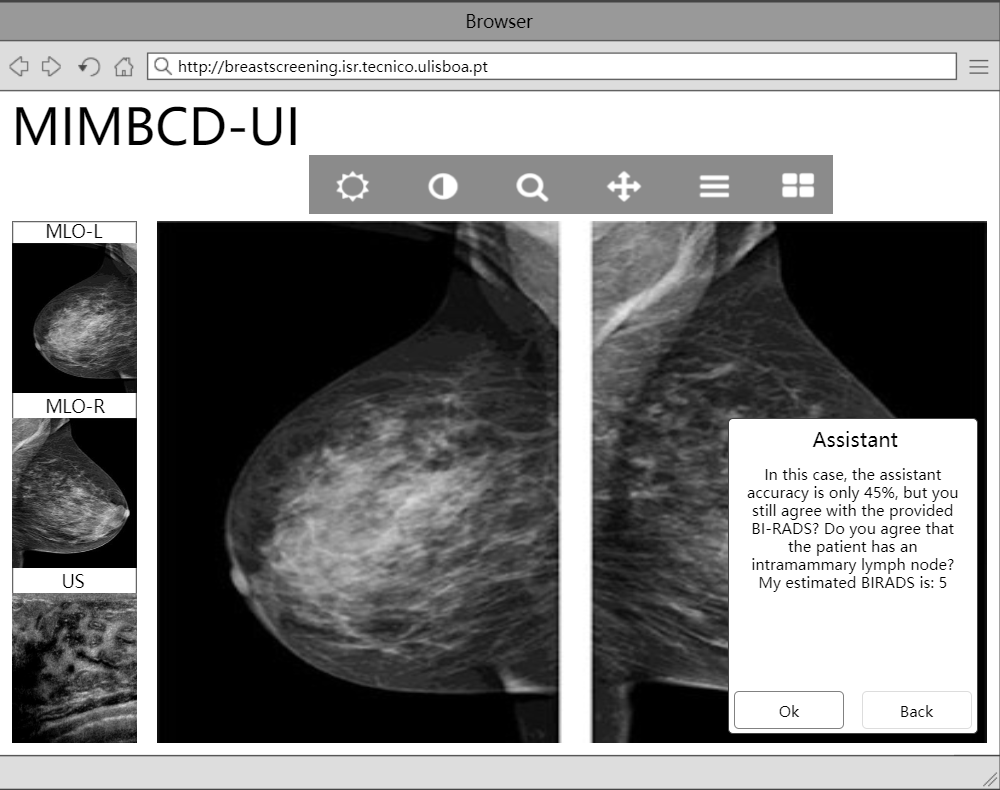
\includegraphics[width=0.40\textwidth]{fig023}
\caption{Example from one of the low-fi prototype views (Figure~\ref{fig:fig022}) for the (b) {\bf Passive} minor scenario. The {\bf Passive} minor scenario was chosen by the clinicians as preferred in comparison to the (a) {\bf Active} minor scenario.}
\label{fig:fig023}
\end{figure}
%%%%%%%%%%%%%%%%%%%%%%%%%%%%%%%%%%%%%%%%%%%%%%%%%%%

To help participants understand and iterate the current status of assertiveness-based assistance, we first asked for clinicians preference concerning an active or passive informing strategy.
Next, we used the \hyperlink{https://www.mockplus.com}{Mockplus} application to create a series of low-fi prototypes (Figure~\ref{fig:fig022}).
Furthermore, we used this application as probe to elicit participants' reactions, critical feedback, and more discussions.
In the end, we asked participants to brainstorm more interactive features that could help them explore and understand an agent assistant.

\subsection{Framework}
\label{sec:sec00602}

The proposed {\it BreastScreening} framework (Figure~\ref{fig:fig008}) will incorporate an {\it AI-Assisted} tool offering clinicians a second opinion during the breast cancer diagnosis that will be accomplished using a DenseNet model~\cite{chen2019learning}.

To validate the proposed DenseNet results, our framework allows the radiologist to {\it accept} or {\it reject} the proposed BI-RADS classification ({\bf MID}) and explanation report ({\bf BED}).
Therefore, the clinician can freely control ({\bf CRD}) the final diagnosis result.
The {\it BreastScreening} platform operates as a website that can be accessed via a web browser.

%%%%%%%%%%%%%%%%%%%%%%%%%%%%%%%%%%%%%%%%%%%%%%%%%%%
\begin{figure}[htbp]
\centering
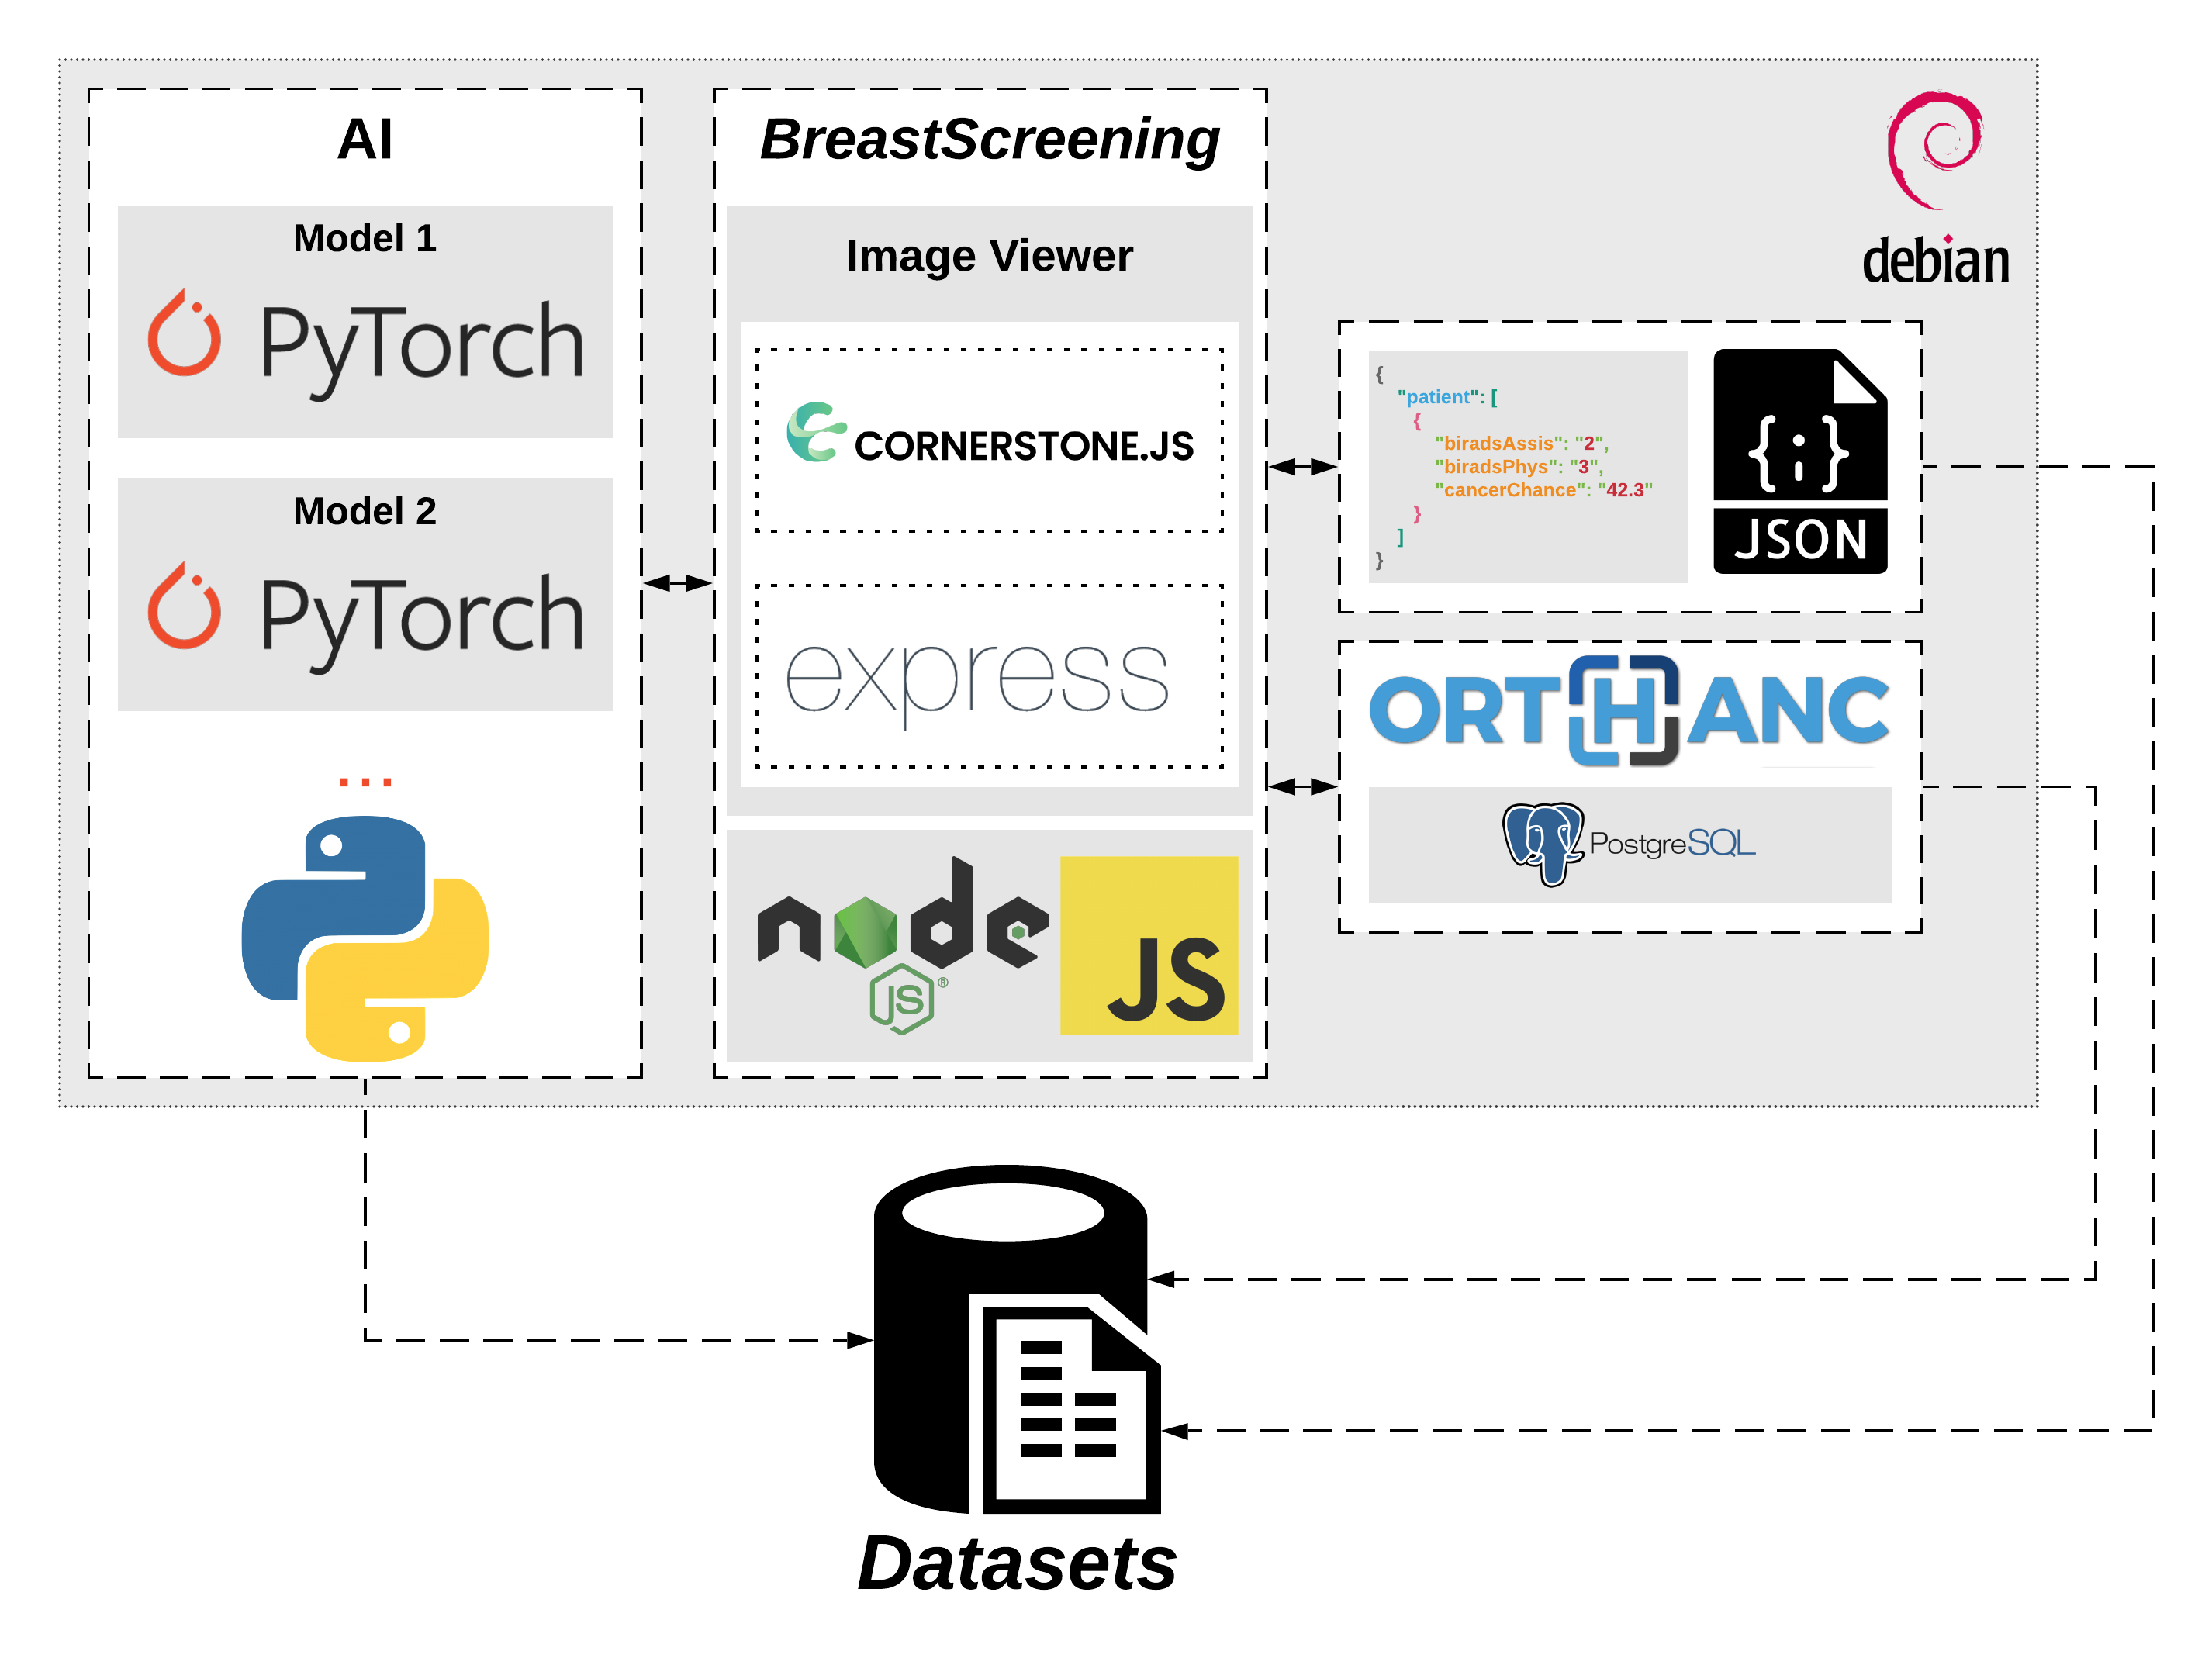
\includegraphics[width=0.45\textwidth]{fig008}
\caption{{\it BreastScreening-AI} Architecture: the main components of the system are AI Application, Image Viewer, Datasets and DICOM Storage. The Image Viewer of {\it BreastScreening} framework will provide essential interaction tools for clinicians. A study list is fetched from the Orthanc server, and through CornerstoneJS the radiologist can manipulate the image, interacting with the assistant at the same time.}
\label{fig:fig008}
\end{figure}
%%%%%%%%%%%%%%%%%%%%%%%%%%%%%%%%%%%%%%%%%%%%%%%%%%%

\subsection{Implementation}
\label{sec:sec00603}

{\it BreastScreening} framework will be implemented using {\it CornerstoneJS}\footnotemark[2]~\cite{urban2017lesiontracker} with a {\it NodeJS}~\cite{10.5555/3002437, drnasin2017javascript} framework\footnotemark[3] and {\it ExpressJS}\footnotemark[4]~\cite{10.1117/12.2285952} for managing the server part.
To feed the system, we will select image sets from \hyperlink{https://hff.min-saude.pt/}{Hospital Fernando Fonseca} and upload them into an {\it Orthanc}~\cite{Jodogne2018} server.

Three imaging modalities (MG, US and MRI) will be provided for each patient.
The images will be pre-processed and anonymized on the {\it Orthanc} server and then consumed by the system.
This system, needs to be efficiently designed as a set of modules (Figure~\ref{fig:fig008}) that can be reused in other imaging applications.

\footnotetext[2]{\hyperlink{https://cornerstonejs.org/}{cornerstonejs.org} - a {\it JavaScript} library to display interactive medical images including but not limited to DICOM. It was used to display the medical images on the browser.}

\footnotetext[3]{\hyperlink{https://nodejs.org}{nodejs.org} - a {\it JavaScript (JS)} based framework for back-end implementation. {\it NodeJS} is defined as a {\it JS} code execution environment.}

\footnotetext[4]{\hyperlink{https://expressjs.com}{expressjs.com} - minimal and flexible {\it NodeJS} web application framework that provides a robust set of features. It deals with requests, responses and subsequent middleware functions.}